\setcounter{chapter}{-1}
\chapter{Thesis Template Information}
\label{ch:template_info}
\section{General}
\label{sec:general}
In total, the Master's thesis (Introduction - Outlook) should amount to \textbf{60 $\pm$ 5 pages} (Bachelor 40 $\pm$ 5) (with 60 being the ideal amount of pages). Recommendations for amount of pages per chapter in case of a Master's thesis and their contents are given for each chapter. Depending on the topic, the distribution between background + related work and own work + evaluation may vary. Ideally, each part should amount to 50\,\%.

The general structure including chapter naming should not be changed unless stated otherwise. The following sections show important information about the general style and formatting and should not be part of the final version!

\section{Notation}
\label{sec:notation}
Please follow the typesetting standards in mathematics that the 'International Standards Organization (ISO) has established. The most important points in it (and some additional) are: 
  

\begin{enumerate}
\item Simple variables are represented by italic letters as $a,\,x,\,A,\,X$.
\item Vectors are written in boldface italic (uncapitalized) as $\vect{a,\, x}$.
\item Matrices may appear as boldface italic capital letters as in $\boldsymbol{A,\, X}$
\item Sets are represented by capital script letters as $\mathcal{A}$, $\mathcal{X}$.
\item Special numbers $\me$, $\mj$ and the differential operator $\diff$ are written in upright roman.
\item Functions are not written in math-mode $\sin(x),\,\operatorname{si}(x)$.
\item Units are separated with half spacing from their value: $5\,\text{m},\,10\,\%,\,\ldots$ 

\item Indexes depending on a variable $i$ are written in math mode $\boldsymbol{a}_i$ while indexes denoting a property are written in usual text $\boldsymbol{a}_{\text{input}}$.

\item If you want to highlight part of your text only use \textit{italicization} and never \underline{underline} or \textbf{embolden} any text (except bold section names, chapters or title or when emphasizing on the best results in tables).

\end{enumerate}

\section{Figures}
\label{sec:figures}                                     

Make sure that you save your graphics in \textit{vector form}, which will not degrade your graphic when magnified. Both eps and pdf support vector graphics. However, saving the file as eps/pdf does \textit{not} guarantee that it is a vector graphic. To make sure zoom in and see if you detect pixels at the text or try to select the text with your cursor. If the text is rasterized (not vectorized) you did a mistake when generating the eps. \autoref{fig:matlabcomp} shows the comparison of a plot once saved as a vector graphic and once as rasterized graphic. 

\begin{figure}[H]
\hfill
	\begin{minipage}{0.4\linewidth}
	\centering
	\subfigure[Matlab plot exported directly as eps/pdf which saves the plot in vector form. Note the nice quality even though it has been rescaled.]{
		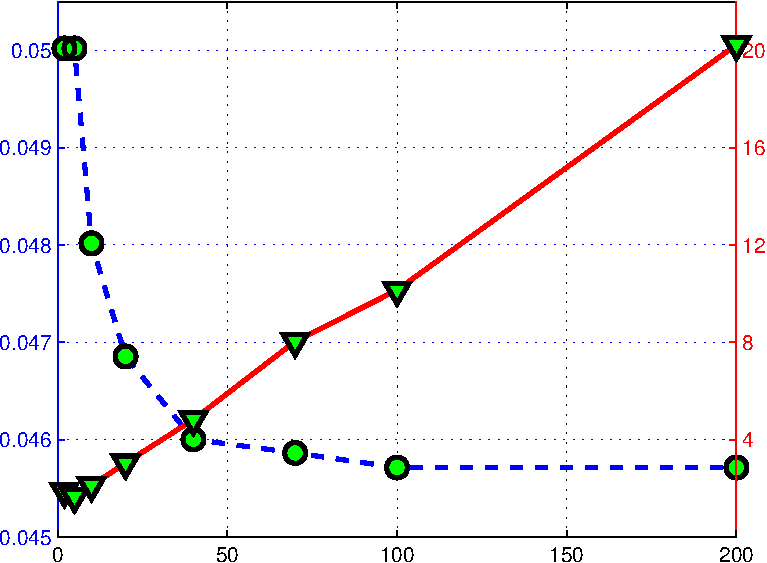
\includegraphics[width=0.9\linewidth]{figures/varyM}
		\label{fig:matlabgood}
	}
	\end{minipage}\hfill
	\begin{minipage}{0.4\linewidth}
	\centering
	\subfigure[Matlab plot saved in bitmap form. The quality is bad. Remember: Export your figures as vector graphic if possible.]{
		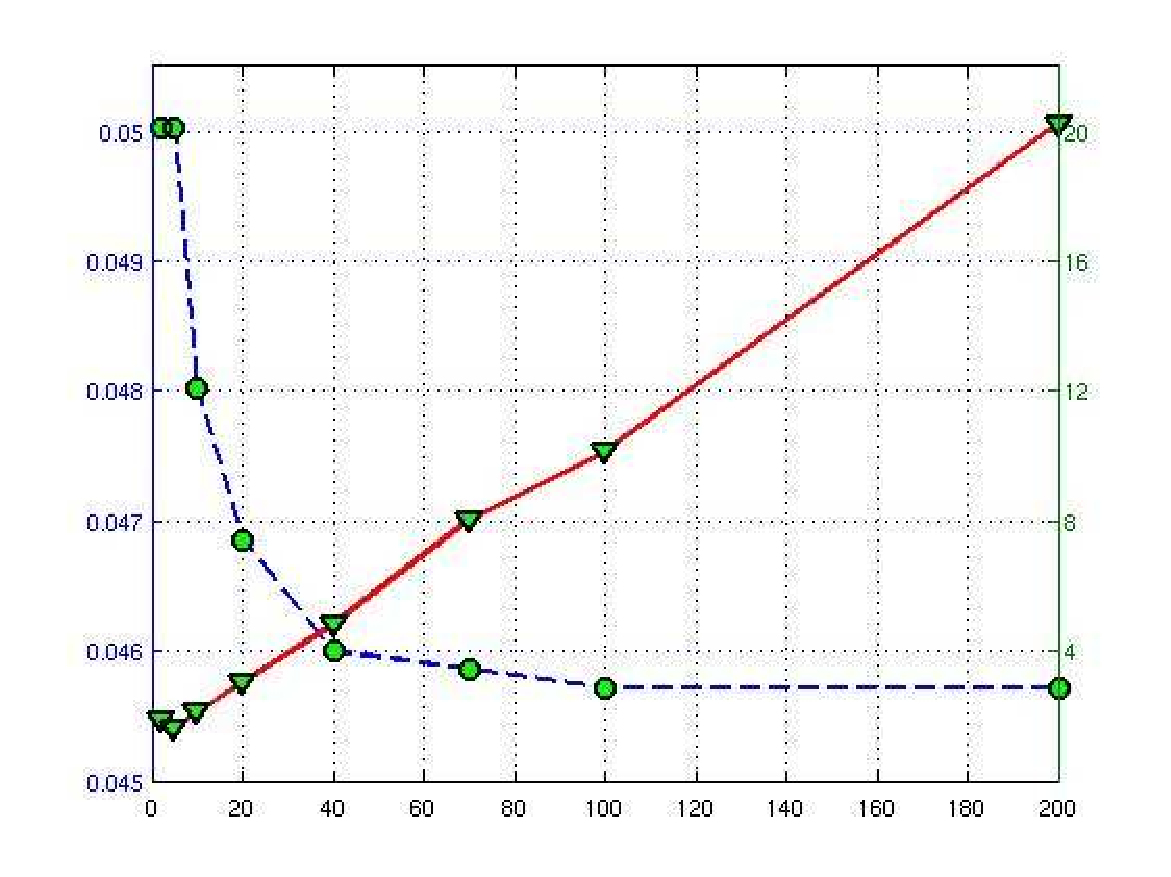
\includegraphics[width=0.9\linewidth]{figures/varyM_jpg}
		\label{fig:matlabbad}
	}
	\end{minipage}
\hfill
	\caption{Comparison of a vector and a rasterized plot.}
	\label{fig:matlabcomp}
\end{figure}


\paragraph*{How to draw high-quality graphics?}
Draw all your drawings with an application that supports vector graphics. My favorite is \textit{Inkscape}. Alternatives include Adobe Illustrator, sK1, yED, Xara Xtreme, OpenOffice Draw. Vector graphics can also directly drawn in latex using tikz notation or with help of TikzEdit.
These applications save your drawing automatically in vector form; if you include a photo it is usually still saved in bitmap form. \autoref{fig:nn} shows a graphic generated in tikz and \autoref{fig:faces} a graphic drawn with Inkscape. Even though a file saved as \textit{.eps} seems to be vectorized, it can also be completely rasterized. To check if your figure is still vectorized zoom in and verify that the text is still sharp. If not you figure might contain transparency or color gradients, which causes \textit{Inkscape} to raster the whole figure.

Make sure all graphics are \textit{well-readable} (line width, colors, fonts, arrows) and \textit{conclusive}. Also, all graphics in your thesis should be \textit{consistent} (same style). As you see in \autoref{fig:nn} and \autoref{fig:faces}, it is hard to create two figures of the same style by using two different tools.

\begin{figure}[H]
  \centering
  \resizebox{.65\textwidth}{!}{
\tikzset{neuron/.style={circle,thick,fill=black!25,minimum size=17pt,inner sep=0pt},
    hidden neuron/.style={neuron,draw,thick, fill=blue!30},
		output neuron/.style={neuron,draw,thick, fill=green!30},
    hoz/.style={rotate=90}}   %<--- for labels
    
    \def\layersep{2.5cm}
    
\begin{tikzpicture}
   \newcommand\Square[1]{+(-#1,-#1) rectangle +(#1,#1)}
   
%%%%%%%%%%%%%%
% Input layer
	\foreach \y / \lab in {1/n,3/j,5/2,6/1}{
	\draw  (0,\y) \Square{3pt} ;    
	\node (I-\y) at (0,\y) {};
	\node  at (-0.5,\y-0.05) {$x_\lab$};
	}

	% Draw dots
	\foreach \y in {2,4}
	\node[hoz]  at (0,\y) {$\dots$};

%%%%%%%%
% Hidden Layer 1
	\foreach \y  in {1,3,4,5}{
	\node[hidden neuron] (H1-\y) at (\layersep,0.5+\y) {};
	}
	% Draw dots
	\foreach \y in {2}
	\node[hoz]  at (\layersep,0.5+\y) {$\dots$};
	
	
	
%%%%%%%
% Connection I - H1
	\foreach \y  in {1,3,5,6}{
		\foreach \yy  in {1,3,4,5}{
		\draw [->, shorten >=0.5pt, thick]  (I-\y.center) -- (H1-\yy) ;
		}
	}
	
	% Draw Squares again
	\foreach \y / \lab in {1/n,3/k,5/2,6/1}
	\draw [fill=white] (0,\y) \Square{3pt} ;    
	

%%%%%%%%
% Hidden Layer 2
	\foreach \y  in {1,3,4}{
	\node[hidden neuron] (H2-\y) at (2*\layersep,1+\y) {};
	}
	% Draw dots
	\foreach \y in {2}
	\node[hoz]  at (2*\layersep,1+\y) {$\dots$};
	
	
	
%%%%%%%
% Connection H1 - H2
	\foreach \y  in {1,3,4,5}{
		\foreach \yy  in {1,3,4}{
		\draw [->, shorten >=0.5pt, thick]  (H1-\y) -- (H2-\yy) ;
		}
	}

	
		

%%%%%%%%
% Hidden Layer 3
	\foreach \y  in {1,3,4}{
	\node[hidden neuron] (H3-\y) at (3*\layersep,1+\y) {};
	}
	% Draw dots
	\foreach \y in {2}
	\node[hoz]  at (3*\layersep,1+\y) {$\dots$};
	
	
	
%%%%%%%
% Connection H2 - H3
	\foreach \y  in {1,3,4}{
		\foreach \yy  in {1,3,4}{
		\draw[-, thick]  (H2-\y) -- ($(H2-\y)!0.75cm!(H3-\yy)$);
		\draw[<-, thick]  (H3-\y) -- ($(H3-\y)!0.75cm!(H2-\yy)$);
		}
	}
	
	% Dots
	% Draw dots
	\foreach \y in {1,2,3,4}
	\node  at (2.5*\layersep,1+\y) {$\dots$};
	

	
	
	
	
	
%%%%%
% Output
	\node [output neuron] (O-1) at (4*\layersep,3.5){};
	
	% Connection
		\foreach \y  in {1,3,4}{
		\draw [->, shorten >=0.5pt, thick]  (H3-\y) -- (O-1) ;
		}
		
		
%%%%%
% Output
	\draw (12.5,3.5) \Square{3pt} ;    
	\node  (OO-1) at  (12.5,3.5) {};
	\node at (13,3.5){$y$};
	\draw [->, shorten >=-0.5pt, thick]  (O-1) -- (OO-1) ;

%%%%%%%%%
% Annotations

	\draw [dashed] (0 * \layersep-25,-0.25) rectangle (0 * \layersep+15,7);
	\draw [dashed] (5 * \layersep-15,-0.25) rectangle (5 * \layersep+25,7);
	\node at (0 * \layersep-5,0) {Inputs};
	\node at (5 * \layersep+5,0) {Output};

\end{tikzpicture}}
  \caption{Multilayer feedforward neural network generated with Tikz.}
  \label{fig:nn}
\end{figure}

\begin{figure}[H]
  \centering
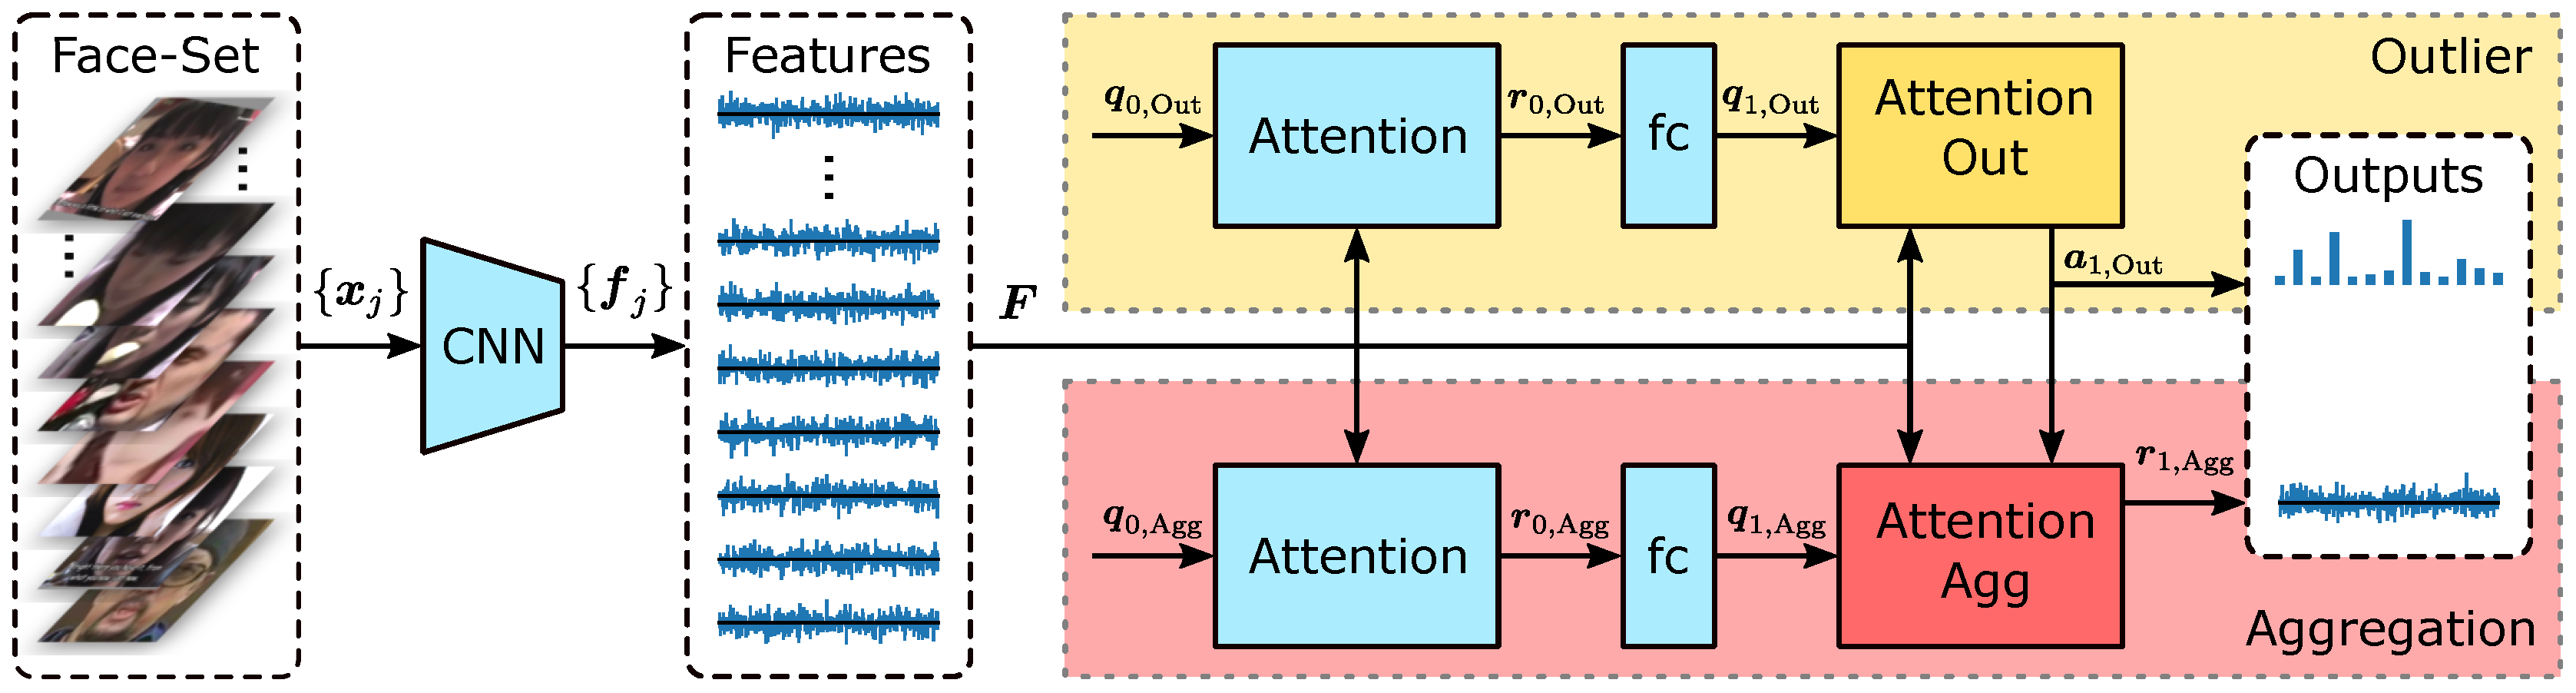
\includegraphics[width=0.87\linewidth]{figures/network.eps}
  \caption{Neural network architecture generated in Inkscape as shown in \cite{hoerman2019ORNAN}.}
  \label{fig:faces}
\end{figure}

\paragraph*{How to generate high-quality plots?}
Python plots (with \textit{matplotlib}) can be converted to tikz code and included in \LaTeX using the package \textit{matplotlib2tikz}.  The huge advantage is that all plots can be edited (labels, limits, ticks, legends, etc.) afterwards within latex without exporting it again. In  \autoref{fig:plot}, you can e.g. adjust the height of the figure by adjusting \verb'\setlength\figureheight{4cm}'. The plot will be generated again with the new height without deforming the text. For MATLAB you can use the script \textit{matlab2tikz}. Do not forget to \textit{label all axes} of your plots and include a \textit{legend}.

\begin{figure}[H]
  \centering
  \newlength\figureheight
\newlength\figurewidth
\setlength\figureheight{4cm}
\setlength\figurewidth{0.7\linewidth}
% This file was created by matplotlib2tikz v0.6.18.

\pgfplotsset{every tick label/.append style={font=\scriptsize}}
\begin{tikzpicture}

\definecolor{color4}{rgb}{0.580392156862745,0.403921568627451,0.741176470588235}
\definecolor{color5}{rgb}{0.549019607843137,0.337254901960784,0.294117647058824}
\definecolor{color2}{rgb}{0.172549019607843,0.627450980392157,0.172549019607843}
\definecolor{color6}{rgb}{0.890196078431372,0.466666666666667,0.76078431372549}
\definecolor{color0}{rgb}{0.12156862745098,0.466666666666667,0.705882352941177}
\definecolor{color1}{rgb}{1,0.498039215686275,0.0549019607843137}
\definecolor{color3}{rgb}{0.83921568627451,0.152941176470588,0.156862745098039}

\begin{groupplot}[group style={group size=2 by 2, vertical sep=50pt,horizontal sep=30pt}, title style={yshift=-1.5ex}]
\nextgroupplot[
height=\figureheight,
tick align=outside,
tick pos=left,
ylabel near ticks,
title={CMC},
width=0.5\figurewidth,
x grid style={white!69.01960784313725!black},
xlabel={Rank},
xmajorgrids,
xminorgrids,
xmin=1, xmax=100,
minor x tick num=10,
xmode=log,
ytick={0.75,0.8,0.85,0.9,0.95,1},
y grid style={white!69.01960784313725!black},
ylabel={TPIR},
ymajorgrids,
ymin=0.75, ymax=1,
every major tick/.style={black, semithick},
yminorgrids,
mark repeat={100}
]
\addplot [thick, color0, dashed, forget plot, mark=pentagon, mark options={solid}]
table [row sep=\\]{%
1	0.886687931404806 \\
2	0.910393874613219 \\
3	0.923837363625459 \\
4	0.930004181108705 \\
5	0.935157965559211 \\
6	0.939029638870805 \\
7	0.942337816075196 \\
8	0.944634278567514 \\
9	0.947085859984341 \\
10	0.94922720355215 \\
11	0.951115288861774 \\
12	0.952544609001202 \\
13	0.954076023436302 \\
14	0.955350224651221 \\
15	0.956577992840633 \\
16	0.957496841501693 \\
17	0.958468714791589 \\
18	0.959081280565629 \\
19	0.959801213918006 \\
20	0.960877818144907 \\
21	0.961744960497798 \\
22	0.962305819963668 \\
23	0.963020480033382 \\
24	0.963324126279071 \\
25	0.964345069235804 \\
26	0.964958953330511 \\
27	0.965367330513204 \\
28	0.965824777362735 \\
29	0.966026329312751 \\
30	0.966383000187274 \\
31	0.966893471665641 \\
32	0.967301848848335 \\
33	0.967507355760347 \\
34	0.967862708314206 \\
35	0.968170309521891 \\
36	0.96837713475457 \\
37	0.968784193616598 \\
38	0.969093113144949 \\
39	0.969349008044466 \\
40	0.96970567891899 \\
41	0.970008006844012 \\
42	0.970312971410367 \\
43	0.970667005643559 \\
44	0.970920263901744 \\
45	0.970971970209913 \\
46	0.97117615880126 \\
47	0.97143073538011 \\
48	0.971581899342622 \\
49	0.972088415858991 \\
50	0.972292604450338 \\
51	0.972600205658024 \\
52	0.972804394249371 \\
53	0.973007264520052 \\
54	0.973110677136391 \\
55	0.973263159419568 \\
56	0.973415641702745 \\
57	0.973619830294092 \\
58	0.973821382244107 \\
59	0.97397518284795 \\
60	0.974282784055636 \\
61	0.974334490363805 \\
62	0.974538678955152 \\
63	0.974640773250826 \\
64	0.974742867546499 \\
65	0.975049150433519 \\
66	0.97530372701237 \\
67	0.975404502987377 \\
68	0.975454890974881 \\
69	0.975505278962385 \\
70	0.975607373258058 \\
71	0.975761173861901 \\
72	0.975912337824412 \\
73	0.975962725811916 \\
74	0.97606482010759 \\
75	0.976217302390767 \\
76	0.976269008698936 \\
77	0.976320715007106 \\
78	0.976372421315276 \\
79	0.976575291585956 \\
80	0.976729092189799 \\
81	0.976829868164807 \\
82	0.976984987089316 \\
83	0.977240881988832 \\
84	0.977240881988832 \\
85	0.977344294605171 \\
86	0.977498095209014 \\
87	0.977651895812857 \\
88	0.977753990108531 \\
89	0.977854766083538 \\
90	0.977905154071042 \\
91	0.978109342662389 \\
92	0.978159730649892 \\
93	0.978363919241239 \\
94	0.978466013536913 \\
95	0.978621132461421 \\
96	0.978723226757095 \\
97	0.978825321052768 \\
98	0.978825321052768 \\
99	0.978927415348442 \\
100	0.979029509644115 \\
};
\addplot [thick, color1, forget plot, mark=x]
table [row sep=\\]{%
1	0.254023056125757 \\
2	0.477712533352731 \\
3	0.624988460786109 \\
4	0.740492995652877 \\
5	0.829493589783004 \\
6	0.879239586387052 \\
7	0.902287557314382 \\
8	0.91239357426538 \\
9	0.918269928709595 \\
10	0.922219674742675 \\
11	0.925595378103225 \\
12	0.928503088048918 \\
13	0.930845983566742 \\
14	0.932935620826382 \\
15	0.934773318148503 \\
16	0.936348528967778 \\
17	0.938176998045238 \\
18	0.939498950606328 \\
19	0.940879201078918 \\
20	0.942411933834684 \\
21	0.943484583099588 \\
22	0.944806535660678 \\
23	0.945677632975567 \\
24	0.946652142906794 \\
25	0.947877274454874 \\
26	0.948489840228915 \\
27	0.949254888286132 \\
28	0.950015981381352 \\
29	0.951088630646255 \\
30	0.95164817179146 \\
31	0.952210349577997 \\
32	0.95307353696889 \\
33	0.953891609654943 \\
34	0.95465665771216 \\
35	0.955316974832373 \\
36	0.956186753826595 \\
37	0.956743658330468 \\
38	0.957047304576157 \\
39	0.957511343029017 \\
40	0.958174296790561 \\
41	0.958682131627597 \\
42	0.959237717810804 \\
43	0.959695164660335 \\
44	0.960149974868535 \\
45	0.960812928630079 \\
46	0.961169599504603 \\
47	0.961530225341125 \\
48	0.961839144869476 \\
49	0.962148064397828 \\
50	0.962402640976679 \\
51	0.962757993530537 \\
52	0.963267146688238 \\
53	0.963521723267088 \\
54	0.963675523870931 \\
55	0.96392746380845 \\
56	0.964284134682974 \\
57	0.964691193545002 \\
58	0.964793287840675 \\
59	0.965099570727695 \\
60	0.965458878243551 \\
61	0.965814230797409 \\
62	0.966070125696925 \\
63	0.966324702275776 \\
64	0.966630985162796 \\
65	0.966835173754143 \\
66	0.967087113691662 \\
67	0.967341690270512 \\
68	0.967545878861859 \\
69	0.967955574365218 \\
70	0.968108056648395 \\
71	0.968463409202253 \\
72	0.968923492693117 \\
73	0.969127681284463 \\
74	0.969538695108488 \\
75	0.969795908328671 \\
76	0.969951027253179 \\
77	0.970002733561349 \\
78	0.970104827857022 \\
79	0.970358086115207 \\
80	0.97081816960607 \\
81	0.97086987591424 \\
82	0.97112445249309 \\
83	0.971227865109429 \\
84	0.971531511355118 \\
85	0.971733063305133 \\
86	0.971935933575814 \\
87	0.971935933575814 \\
88	0.972036709550822 \\
89	0.972138803846495 \\
90	0.972443768412849 \\
91	0.972544544387857 \\
92	0.97264663868353 \\
93	0.972800439287373 \\
94	0.972901215262381 \\
95	0.973157110161897 \\
96	0.973207498149401 \\
97	0.973257886136905 \\
98	0.973309592445074 \\
99	0.973463393048917 \\
100	0.973566805665256 \\
};
\addplot [thick, color2, forget plot, mark=+]
table [row sep=\\]{%
1	0.798470992933072 \\
2	0.859851341367829 \\
3	0.885433504999874 \\
4	0.897350852859677 \\
5	0.906937170087648 \\
6	0.912499331720848 \\
7	0.917495360605515 \\
8	0.920859199080073 \\
9	0.924528002120985 \\
10	0.927129429179657 \\
11	0.930287760742203 \\
12	0.933355862895068 \\
13	0.936203956608596 \\
14	0.938138474943726 \\
15	0.940128654549024 \\
16	0.94160704435529 \\
17	0.94344474167741 \\
18	0.944765375917835 \\
19	0.946042213774085 \\
20	0.94757230988852 \\
21	0.948794804795269 \\
22	0.949868772380838 \\
23	0.951042197620749 \\
24	0.952064458898149 \\
25	0.953548121987077 \\
26	0.954364876352464 \\
27	0.955125969447684 \\
28	0.955735898580393 \\
29	0.956702498587625 \\
30	0.957110875770319 \\
31	0.957923675173708 \\
32	0.958332052356402 \\
33	0.959046712426115 \\
34	0.959350358671804 \\
35	0.959859511829505 \\
36	0.960217501024695 \\
37	0.960575490219884 \\
38	0.961136349685755 \\
39	0.961848373114137 \\
40	0.962358844592504 \\
41	0.962822883045364 \\
42	0.963127847611719 \\
43	0.96358529446125 \\
44	0.96389157734827 \\
45	0.964295999568966 \\
46	0.964703058430994 \\
47	0.965006704676683 \\
48	0.965314305884369 \\
49	0.96572663802906 \\
50	0.966133696891087 \\
51	0.966337885482434 \\
52	0.966592462061284 \\
53	0.966897426627639 \\
54	0.967203709514659 \\
55	0.967763250659864 \\
56	0.968069533546884 \\
57	0.968272403817565 \\
58	0.968322791805069 \\
59	0.968529617037747 \\
60	0.968835899924767 \\
61	0.969189934157959 \\
62	0.969395441069972 \\
63	0.969757385227159 \\
64	0.970111419460352 \\
65	0.970315608051698 \\
66	0.970315608051698 \\
67	0.970518478322379 \\
68	0.970673597246888 \\
69	0.970826079530065 \\
70	0.971028949800746 \\
71	0.971282208058931 \\
72	0.971636242292123 \\
73	0.971892137191639 \\
74	0.971992913166647 \\
75	0.972096325782986 \\
76	0.972405245311338 \\
77	0.972507339607011 \\
78	0.972761916185862 \\
79	0.972964786456543 \\
80	0.973118587060386 \\
81	0.973168975047889 \\
82	0.973321457331067 \\
83	0.973577352230583 \\
84	0.97372983451376 \\
85	0.97403611740078 \\
86	0.9743424002878 \\
87	0.97444581290414 \\
88	0.974496200891643 \\
89	0.974496200891643 \\
90	0.974598295187317 \\
91	0.97464868317482 \\
92	0.974749459149828 \\
93	0.974799847137332 \\
94	0.974952329420509 \\
95	0.97515519969119 \\
96	0.975309000295033 \\
97	0.975462800898876 \\
98	0.975615283182053 \\
99	0.975769083785896 \\
100	0.975872496402235 \\
};
\addplot [thick, color3, forget plot, mark=diamond]
table [row sep=\\]{%
1	0.82894709115411 \\
2	0.867659577505844 \\
3	0.885416075029016 \\
4	0.895348516566184 \\
5	0.903350394730219 \\
6	0.909209611005779 \\
7	0.914108818877435 \\
8	0.919151280787607 \\
9	0.922914268200198 \\
10	0.92587368445406 \\
11	0.928939149965593 \\
12	0.931537940382934 \\
13	0.934085024492105 \\
14	0.935757056324391 \\
15	0.937789713993197 \\
16	0.939016163861944 \\
17	0.941409447367272 \\
18	0.942480778311509 \\
19	0.943603815563917 \\
20	0.944374136903797 \\
21	0.945601905093209 \\
22	0.946671917716781 \\
23	0.947435647453333 \\
24	0.948613027655241 \\
25	0.949685676920144 \\
26	0.950803440889888 \\
27	0.952275239092824 \\
28	0.953038968829376 \\
29	0.953854404874097 \\
30	0.954766661931829 \\
31	0.95553039166838 \\
32	0.956092569454917 \\
33	0.956600404291952 \\
34	0.957214288386658 \\
35	0.95741979529867 \\
36	0.957981973085207 \\
37	0.95874833946309 \\
38	0.959204467991956 \\
39	0.959661914841487 \\
40	0.960068973703515 \\
41	0.960373938269869 \\
42	0.960938752697737 \\
43	0.961295423572261 \\
44	0.961748915459795 \\
45	0.961901397742972 \\
46	0.96236016291317 \\
47	0.962718152108359 \\
48	0.963023116674714 \\
49	0.96322730526606 \\
50	0.963684752115592 \\
51	0.963888940706939 \\
52	0.964094447618951 \\
53	0.964297317889632 \\
54	0.96439809386464 \\
55	0.964856859034837 \\
56	0.965061047626184 \\
57	0.965163141921857 \\
58	0.965468106488212 \\
59	0.96562322541272 \\
60	0.965879120312237 \\
61	0.966083308903583 \\
62	0.966337885482434 \\
63	0.966542074073781 \\
64	0.966847038640135 \\
65	0.967101615218986 \\
66	0.96740657978534 \\
67	0.96771286267236 \\
68	0.967917051263707 \\
69	0.968224652471393 \\
70	0.968275040458896 \\
71	0.968326746767066 \\
72	0.968427522742074 \\
73	0.968580005025251 \\
74	0.968835899924767 \\
75	0.969139546170456 \\
76	0.96944451073681 \\
77	0.96975079362383 \\
78	0.969802499932 \\
79	0.969852887919503 \\
80	0.97010878281902 \\
81	0.970514523360382 \\
82	0.970668323964225 \\
83	0.970819487926736 \\
84	0.971076701146918 \\
85	0.971279571417599 \\
86	0.971380347392607 \\
87	0.971636242292123 \\
88	0.971686630279627 \\
89	0.97184043088347 \\
90	0.971941206858477 \\
91	0.972145395449824 \\
92	0.972399972028675 \\
93	0.972605478940687 \\
94	0.972657185248857 \\
95	0.972809667532034 \\
96	0.972913080148373 \\
97	0.973016492764712 \\
98	0.973168975047889 \\
99	0.973426188268072 \\
100	0.97358130719258 \\
};
\addplot [thick, color0, forget plot, mark=pentagon]
table [row sep=\\]{%
1	0.709391007760792 \\
2	0.778013167782827 \\
3	0.799781956014778 \\
4	0.812029316533586 \\
5	0.821054774295686 \\
6	0.82768299359046 \\
7	0.833341976236671 \\
8	0.837590095232775 \\
9	0.841932398600558 \\
10	0.846314543390519 \\
11	0.850186216702112 \\
12	0.853292841956488 \\
13	0.855688762103148 \\
14	0.857777081042121 \\
15	0.859620051646906 \\
16	0.861966902126727 \\
17	0.863801962807517 \\
18	0.865231282946944 \\
19	0.866866109998384 \\
20	0.868703807320504 \\
21	0.870335997730613 \\
22	0.871717566523868 \\
23	0.87340014492148 \\
24	0.874678301098396 \\
25	0.875947229030651 \\
26	0.876974763590714 \\
27	0.8782463281643 \\
28	0.879215564812865 \\
29	0.880184801461429 \\
30	0.881409933009509 \\
31	0.882733203891266 \\
32	0.883601664564822 \\
33	0.884525786508546 \\
34	0.885190058590756 \\
35	0.885907355301801 \\
36	0.886518602755175 \\
37	0.887027755912877 \\
38	0.887845828598929 \\
39	0.888710334310489 \\
40	0.889727322305225 \\
41	0.890288181771095 \\
42	0.890948498891308 \\
43	0.891763934936029 \\
44	0.892121924131219 \\
45	0.892783559572097 \\
46	0.893241006421629 \\
47	0.894263267699028 \\
48	0.894822808844233 \\
49	0.895280255693764 \\
50	0.895992279122146 \\
51	0.896858103154371 \\
52	0.897316868324569 \\
53	0.897928115777943 \\
54	0.898441223897642 \\
55	0.898797894772166 \\
56	0.89935743591737 \\
57	0.899612012496221 \\
58	0.900276284578431 \\
59	0.900944511622638 \\
60	0.901606147063516 \\
61	0.902015842566876 \\
62	0.902523677403911 \\
63	0.902982442574108 \\
64	0.903389501436136 \\
65	0.904049818556348 \\
66	0.904407807751538 \\
67	0.905121149500586 \\
68	0.905375726079436 \\
69	0.905682008966456 \\
70	0.906036043199649 \\
71	0.906496126690512 \\
72	0.90710605582322 \\
73	0.90746404501841 \\
74	0.907766372943433 \\
75	0.90817343180546 \\
76	0.90853142100065 \\
77	0.908890728516506 \\
78	0.909246081070364 \\
79	0.910062835435751 \\
80	0.910419506310275 \\
81	0.910776177184799 \\
82	0.911033390404981 \\
83	0.911289285304497 \\
84	0.911956194028039 \\
85	0.912414959198236 \\
86	0.912926748997269 \\
87	0.913133574229947 \\
88	0.913438538796301 \\
89	0.913895985645833 \\
90	0.914153198866015 \\
91	0.914561576048708 \\
92	0.914867858935729 \\
93	0.915326624105926 \\
94	0.915735001288619 \\
95	0.915941826521298 \\
96	0.916146015112644 \\
97	0.916452297999665 \\
98	0.916604780282842 \\
99	0.916706874578515 \\
100	0.917015794106867 \\
};
\addplot [thick, color4, forget plot, mark=o]
table [row sep=\\]{%
1	0.846311031342579 \\
2	0.885611035375702 \\
3	0.900369593543501 \\
4	0.908934967814738 \\
5	0.915038214103822 \\
6	0.920283546284675 \\
7	0.923860801595241 \\
8	0.927626425649164 \\
9	0.930632274928532 \\
10	0.933642079169898 \\
11	0.935526209517525 \\
12	0.936951574694955 \\
13	0.938382213155048 \\
14	0.939602071420465 \\
15	0.940974411969059 \\
16	0.94265435372534 \\
17	0.943675296682074 \\
18	0.944546393996962 \\
19	0.945567336953695 \\
20	0.946431842665255 \\
21	0.947499218647495 \\
22	0.94836504267972 \\
23	0.949383348995122 \\
24	0.949991959807165 \\
25	0.951114997059572 \\
26	0.95182833880862 \\
27	0.952794938815852 \\
28	0.953200679357214 \\
29	0.953920612709591 \\
30	0.954632636137973 \\
31	0.954887212716823 \\
32	0.955547529837036 \\
33	0.956462423536099 \\
34	0.956817776089957 \\
35	0.95727785958082 \\
36	0.957736624751017 \\
37	0.958449966500065 \\
38	0.958959119657766 \\
39	0.959163308249113 \\
40	0.959624710060642 \\
41	0.959777192343819 \\
42	0.960131226577011 \\
43	0.960387121476527 \\
44	0.960641698055378 \\
45	0.961050075238072 \\
46	0.961410701074593 \\
47	0.961612253024608 \\
48	0.961866829603458 \\
49	0.961917217590962 \\
50	0.962069699874139 \\
51	0.962273888465486 \\
52	0.962629241019344 \\
53	0.962984593573202 \\
54	0.963289558139557 \\
55	0.963392970755896 \\
56	0.963646229014081 \\
57	0.963798711297258 \\
58	0.964054606196774 \\
59	0.964156700492448 \\
60	0.964409958750632 \\
61	0.964614147341979 \\
62	0.964867405600164 \\
63	0.965070275870845 \\
64	0.965221439833356 \\
65	0.965478653053538 \\
66	0.965835323928062 \\
67	0.965835323928062 \\
68	0.965937418223735 \\
69	0.966088582186247 \\
70	0.96619067648192 \\
71	0.966445253060771 \\
72	0.966597735343948 \\
73	0.966750217627125 \\
74	0.966852311922798 \\
75	0.967057818834811 \\
76	0.967264644067489 \\
77	0.967315032054993 \\
78	0.967365420042497 \\
79	0.967517902325674 \\
80	0.967720772596355 \\
81	0.967874573200198 \\
82	0.967976667495871 \\
83	0.968129149779048 \\
84	0.968232562395388 \\
85	0.968282950382891 \\
86	0.96848977561557 \\
87	0.968692645886251 \\
88	0.968996292131939 \\
89	0.969303893339625 \\
90	0.969355599647795 \\
91	0.969508081930972 \\
92	0.969710952201653 \\
93	0.970017235088673 \\
94	0.970068941396843 \\
95	0.970119329384346 \\
96	0.970273129988189 \\
97	0.970375224283863 \\
98	0.970426930592032 \\
99	0.970578094554544 \\
100	0.970628482542047 \\
};
\addplot [thick, color5, forget plot, mark=triangle]
table [row sep=\\]{%
1	0.857988304150855 \\
2	0.89041605887568 \\
3	0.904393749138272 \\
4	0.913148810473531 \\
5	0.919269194931271 \\
6	0.924255995571276 \\
7	0.928331857474216 \\
8	0.931901202860787 \\
9	0.934656430523302 \\
10	0.936842888795952 \\
11	0.93822050262721 \\
12	0.939442997533959 \\
13	0.940865726070057 \\
14	0.942706060033509 \\
15	0.943723048028246 \\
16	0.94494686125566 \\
17	0.946120286495571 \\
18	0.946934404219627 \\
19	0.947798909931186 \\
20	0.948668688925408 \\
21	0.949640562215304 \\
22	0.950457316580691 \\
23	0.951624150217273 \\
24	0.952540362237001 \\
25	0.953302773652887 \\
26	0.953864951439424 \\
27	0.954472243930801 \\
28	0.955184267359183 \\
29	0.955540938233707 \\
30	0.956202573674585 \\
31	0.95676211481979 \\
32	0.957065761065478 \\
33	0.957677008518853 \\
34	0.958236549664057 \\
35	0.958542832551078 \\
36	0.958902140066933 \\
37	0.959413929865966 \\
38	0.959974789331836 \\
39	0.96007688362751 \\
40	0.960430917860702 \\
41	0.960735882427056 \\
42	0.960990459005907 \\
43	0.961296741892927 \\
44	0.961499612163608 \\
45	0.961804576729962 \\
46	0.962159929283821 \\
47	0.962260705258828 \\
48	0.962616057812686 \\
49	0.962922340699706 \\
50	0.963329399561734 \\
51	0.963481881844911 \\
52	0.963992353323278 \\
53	0.964195223593959 \\
54	0.964606237417984 \\
55	0.964761356342493 \\
56	0.964964226613174 \\
57	0.965067639229513 \\
58	0.96527182782086 \\
59	0.965627180374718 \\
60	0.965678886682887 \\
61	0.965985169569908 \\
62	0.966136333532419 \\
63	0.966340522123766 \\
64	0.966544710715112 \\
65	0.966595098702616 \\
66	0.966799287293963 \\
67	0.96700347588531 \\
68	0.967155958168487 \\
69	0.967360146759834 \\
70	0.967462241055507 \\
71	0.967565653671846 \\
72	0.967769842263193 \\
73	0.967821548571362 \\
74	0.967923642867036 \\
75	0.968278995420894 \\
76	0.968533571999744 \\
77	0.96884117320743 \\
78	0.969044043478111 \\
79	0.969245595428126 \\
80	0.9693476897238 \\
81	0.969603584623316 \\
82	0.969704360598324 \\
83	0.969754748585828 \\
84	0.96990854918967 \\
85	0.970009325164678 \\
86	0.970110101139686 \\
87	0.970365996039202 \\
88	0.970673597246888 \\
89	0.970824761209399 \\
90	0.970975925171911 \\
91	0.971127089134422 \\
92	0.971280889738265 \\
93	0.971434690342108 \\
94	0.971536784637781 \\
95	0.971690585241624 \\
96	0.971792679537298 \\
97	0.971947798461806 \\
98	0.972048574436814 \\
99	0.972254081348827 \\
100	0.97230446933633 \\
};
\addplot [thick, color6, forget plot, mark=oplus]
table [row sep=\\]{%
1	0.863435188281724 \\
2	0.893510819244064 \\
3	0.906520591178757 \\
4	0.914875185255318 \\
5	0.919721368498139 \\
6	0.924661736112638 \\
7	0.928380927141054 \\
8	0.932057640105962 \\
9	0.935166902001669 \\
10	0.937508479198828 \\
11	0.939187102634442 \\
12	0.940051608346002 \\
13	0.941071232982069 \\
14	0.942858542316686 \\
15	0.944233519506612 \\
16	0.945357875079685 \\
17	0.9465816883071 \\
18	0.947391851069158 \\
19	0.948152944164378 \\
20	0.949173887121112 \\
21	0.949895138794155 \\
22	0.950662823492703 \\
23	0.951681129808106 \\
24	0.952645093174006 \\
25	0.953357116602389 \\
26	0.954071776672102 \\
27	0.954627362855309 \\
28	0.955599236145205 \\
29	0.95590420071156 \\
30	0.956515448164934 \\
31	0.957076307630805 \\
32	0.957178401926478 \\
33	0.957940813342364 \\
34	0.958297484216888 \\
35	0.958655473412078 \\
36	0.959063850594771 \\
37	0.959421839789961 \\
38	0.959726804356315 \\
39	0.960030450602004 \\
40	0.960384484835196 \\
41	0.960688131080884 \\
42	0.96099573228857 \\
43	0.961148214571747 \\
44	0.96130201517559 \\
45	0.961454497458768 \\
46	0.961707755716952 \\
47	0.96180853169196 \\
48	0.962163884245818 \\
49	0.962264660220825 \\
50	0.962825519686696 \\
51	0.9628759076742 \\
52	0.963232578548724 \\
53	0.963435448819405 \\
54	0.963845144322764 \\
55	0.964102357542946 \\
56	0.964356934121797 \\
57	0.964562441033809 \\
58	0.964763992983825 \\
59	0.964915156946336 \\
60	0.965018569562675 \\
61	0.965323534129029 \\
62	0.96552640439971 \\
63	0.965677568362222 \\
64	0.965933463261738 \\
65	0.966036875878077 \\
66	0.966188039840588 \\
67	0.966392228431935 \\
68	0.966442616419439 \\
69	0.966646805010786 \\
70	0.966801923935295 \\
71	0.967057818834811 \\
72	0.967413171388669 \\
73	0.967515265684342 \\
74	0.967669066288185 \\
75	0.96792232454637 \\
76	0.968176901125221 \\
77	0.96822860743339 \\
78	0.968434114345403 \\
79	0.968636984616084 \\
80	0.968688690924253 \\
81	0.96884117320743 \\
82	0.968994973811273 \\
83	0.969097068106947 \\
84	0.969249550390124 \\
85	0.969350326365132 \\
86	0.969502808648309 \\
87	0.96970567891899 \\
88	0.969961573818506 \\
89	0.970062349793513 \\
90	0.970265220064194 \\
91	0.970466772014209 \\
92	0.970670960605556 \\
93	0.970722666913726 \\
94	0.970774373221895 \\
95	0.970928173825738 \\
96	0.971081974429581 \\
97	0.971235775033424 \\
98	0.971386938995936 \\
99	0.971540739599779 \\
100	0.971591127587282 \\
};
\nextgroupplot[
height=\figureheight,
legend cell align={left},
legend entries={{optimal},{Baseline 1},{Baseline 2},{Baseline 3},{Baseline 4},{Baseline 5},{Ours 1},{Ours 2}},
legend columns=4, 
legend style={
at={(-0.2,-0.7)}, 
anchor=center, 
font=\scriptsize,
/tikz/every even column/.append style={column sep=0.2cm},
draw=white!80.0!black},
tick align=outside,
tick pos=left,
title={IET},
width=0.5\figurewidth,
x grid style={lightgray!92.02614379084967!black},
xlabel={FPIR},
xmajorgrids,
xmin=0.001, xmax=1,
xminorgrids,
xmode=log,
y grid style={lightgray!92.02614379084967!black},
%ylabel={TPIR},
ytick={0.01,0.1,1},
yticklabels={0.01,0.1,1},
ymajorgrids,
every major tick/.style={black, semithick},
ymin=0.01, ymax=1,
yminorgrids,
ymode=log,
mark repeat={100}
]
\addlegendimage{color0, thick, dashed, mark=pentagon, mark options={solid}}
\addlegendimage{color1, thick, mark=x}
\addlegendimage{color2, thick, mark=+}
\addlegendimage{color3, thick, mark=diamond}
\addlegendimage{color0, thick, mark=pentagon}
\addlegendimage{color4, thick, mark=o}
\addlegendimage{color5, thick, mark=triangle}
\addlegendimage{color6, thick, mark=oplus}
\addplot [thick, color0, dashed, mark=pentagon, mark options={solid}]
table [row sep=\\]{%
0	0 \\
0	0 \\
0	0 \\
0	0 \\
0	0 \\
0	0.000102094295673316 \\
0	0.000204188591346743 \\
0	0.000509153157701059 \\
0	0.00101698799473626 \\
0	0.00132458920242229 \\
0	0.00167994175628039 \\
0	0.0026929747890192 \\
0	0.00370732614242386 \\
0	0.00477338380399817 \\
0	0.00685642946030862 \\
0	0.0096554535069987 \\
0	0.0130206103022227 \\
0	0.017360277028674 \\
0	0.0219969983974848 \\
0	0.0292338285043021 \\
0	0.0379424568140556 \\
0	0.0497788035088381 \\
0	0.0640865064304348 \\
0	0.080107109124957 \\
0	0.0990818547906783 \\
0	0.119142724730164 \\
0	0.146271830843097 \\
5.03879875037791e-05	0.176483832438421 \\
5.03879875037791e-05	0.207871604112785 \\
0.000151163962511337	0.242510573400708 \\
0.000151163962511337	0.277933047235169 \\
0.000354034233192271	0.312780160076435 \\
0.000454810208199829	0.351151503599432 \\
0.000454810208199829	0.386615428978939 \\
0.000811481082723736	0.424480547787769 \\
0.000811481082723736	0.464173843871857 \\
0.000913575378397112	0.50475068576123 \\
0.00137102222792858	0.5413547865618 \\
0.00218645827264977	0.5790463299568 \\
0.00330290392172781	0.615511423483053 \\
0.0054468841308687	0.647303909180316 \\
0.0102242228968643	0.678889569644901 \\
0.0158380908382341	0.711264007938687 \\
0.0256803029657213	0.7392259800672 \\
0.0410830666035401	0.764164964747688 \\
0.0664818429726891	0.787069973438705 \\
0.104742890473815	0.809616992934531 \\
0.151489921204026	0.829986782402368 \\
0.219061259808071	0.846250388591951 \\
0.301423088078098	0.860822188139262 \\
0.402918001184092	0.875466787125395 \\
0.518623796198672	0.888565470149104 \\
0.635572152732191	0.902026097329999 \\
0.748844088103005	0.915794325718581 \\
0.844636805783019	0.926412132468612 \\
0.918683730286807	0.936108453916251 \\
0.963161540344625	0.944309247388969 \\
0.987927241413486	0.951030332734757 \\
0.996803145335943	0.956495673354947 \\
0.99969371711298	0.962089766486329 \\
0.999897905704327	0.965814230797409 \\
1	0.969066746731633 \\
1	0.970753280091242 \\
1	0.971930660293151 \\
1	0.972189191833999 \\
1	0.972292604450338 \\
1	0.972292604450338 \\
1	0.972292604450338 \\
1	0.972292604450338 \\
1	0.972292604450338 \\
1	0.972292604450338 \\
1	0.972292604450338 \\
1	0.972292604450338 \\
1	0.972292604450338 \\
1	0.972292604450338 \\
1	0.972292604450338 \\
1	0.972292604450338 \\
1	0.972292604450338 \\
1	0.972292604450338 \\
1	0.972292604450338 \\
1	0.972292604450338 \\
1	0.972292604450338 \\
1	0.972292604450338 \\
1	0.972292604450338 \\
1	0.972292604450338 \\
1	0.972292604450338 \\
1	0.972292604450338 \\
1	0.972292604450338 \\
1	0.972292604450338 \\
1	0.972292604450338 \\
1	0.972292604450338 \\
1	0.972292604450338 \\
1	0.972292604450338 \\
1	0.972292604450338 \\
1	0.972292604450338 \\
1	0.972292604450338 \\
1	0.972292604450338 \\
1	0.972292604450338 \\
1	0.972292604450338 \\
1	0.972292604450338 \\
};
\addplot [thick, color1, mark=x]
table [row sep=\\]{%
0	0 \\
0.689380525808811	0 \\
0.689380525808811	0.000201551950015144 \\
0.689380525808811	0.000664272082209871 \\
0.689380525808811	0.00182715075679418 \\
0.689380525808811	0.00442462285346912 \\
0.689380525808811	0.00990871176518349 \\
0.689380525808811	0.0168672355211655 \\
0.689380525808811	0.0233617208242871 \\
0.689380525808811	0.0284585256839609 \\
0.689380525808811	0.032737257857582 \\
0.689380525808811	0.0368595527860285 \\
0.689380525808811	0.0396704417187108 \\
0.689380525808811	0.0432160573332967 \\
0.689380525808811	0.047374238721923 \\
0.689380525808811	0.0507911018253165 \\
0.689380525808811	0.0554676646163046 \\
0.689380525808811	0.060552604589986 \\
0.689380525808811	0.0651906442794628 \\
0.689380525808811	0.0718850714097309 \\
0.689380525808811	0.0772776125910983 \\
0.68943223211698	0.0855011093173381 \\
0.68948393842515	0.0916455153492648 \\
0.68948393842515	0.100118023569489 \\
0.68948393842515	0.108729830866233 \\
0.68948393842515	0.120192076715633 \\
0.68948393842515	0.136125378444009 \\
0.68948393842515	0.154502351665216 \\
0.68948393842515	0.176183255326615 \\
0.68948393842515	0.203888014234945 \\
0.68948393842515	0.236357663418873 \\
0.68948393842515	0.270032669340895 \\
0.68948393842515	0.303822952765248 \\
0.689685490375165	0.345612185910101 \\
0.689787584670838	0.386384722862421 \\
0.690246349841036	0.425735849599309 \\
0.690348444136709	0.470265808879353 \\
0.690961009910749	0.513853189726353 \\
0.691369387093443	0.55460463354802 \\
0.692591882000192	0.596557479145782 \\
0.694681519259831	0.636868906088776 \\
0.698756062842105	0.674646432129257 \\
0.702438049089676	0.711320695727317 \\
0.709393644402124	0.746160190446792 \\
0.720214321422836	0.77697845801503 \\
0.735429008119501	0.802470392237394 \\
0.755765547768489	0.827160073621696 \\
0.779965850805077	0.849803914130532 \\
0.808823968341128	0.870856723972103 \\
0.843631531562421	0.88878547858844 \\
0.87886622025793	0.901803160447128 \\
0.912396945622972	0.914954868099673 \\
0.94376259764822	0.927609287480508 \\
0.969344761280265	0.937585525401851 \\
0.9850702112575	0.944959017943855 \\
0.993793341094577	0.949899385558355 \\
0.998225873872041	0.954179436052642 \\
0.999746741741815	0.957085827677668 \\
0.999949612012496	0.959488339427657 \\
1	0.961274330441608 \\
1	0.961836508228145 \\
1	0.962195815744 \\
1	0.962299228360339 \\
1	0.962402640976679 \\
1	0.962402640976679 \\
1	0.962402640976679 \\
1	0.962402640976679 \\
1	0.962402640976679 \\
1	0.962402640976679 \\
1	0.962402640976679 \\
1	0.962402640976679 \\
1	0.962402640976679 \\
1	0.962402640976679 \\
1	0.962402640976679 \\
1	0.962402640976679 \\
1	0.962402640976679 \\
1	0.962402640976679 \\
1	0.962402640976679 \\
1	0.962402640976679 \\
1	0.962402640976679 \\
1	0.962402640976679 \\
1	0.962402640976679 \\
1	0.962402640976679 \\
1	0.962402640976679 \\
1	0.962402640976679 \\
1	0.962402640976679 \\
1	0.962402640976679 \\
1	0.962402640976679 \\
1	0.962402640976679 \\
1	0.962402640976679 \\
1	0.962402640976679 \\
1	0.962402640976679 \\
1	0.962402640976679 \\
1	0.962402640976679 \\
1	0.962402640976679 \\
1	0.962402640976679 \\
1	0.962402640976679 \\
1	0.962402640976679 \\
1	0.962402640976679 \\
1	0.962402640976679 \\
};
\addplot [thick, color2, mark=+]
table [row sep=\\]{%
0	0 \\
0	0 \\
0	0 \\
0	0 \\
0	0 \\
0	5.17063081695301e-05 \\
0	0.000153800603842957 \\
0	0.000458765170197273 \\
0	0.000763729736551588 \\
0	0.00086714235289076 \\
0	0.000969236648564187 \\
0	0.00107133094423761 \\
0	0.00112303725240714 \\
0	0.00112303725240714 \\
0	0.00127551953558425 \\
0	0.00142800181876146 \\
0	0.00147838980626525 \\
0	0.00158180242260442 \\
0	0.00173428470578152 \\
0	0.00193847329712837 \\
0	0.00209227390097122 \\
0	0.00234421383849015 \\
0	0.00264786008417861 \\
0	0.00295150632986718 \\
0	0.00325778921688724 \\
0	0.00371655438708463 \\
0	0.00428136881495267 \\
0	0.00479315861398544 \\
0	0.00570409735105093 \\
0	0.0068709309876327 \\
0	0.00778450636602979 \\
0	0.0088028126814319 \\
0	0.0105384157078793 \\
0	0.0123721580680026 \\
0	0.0148276944468269 \\
0	0.0178892049963624 \\
0	0.0226543870741629 \\
5.03879875037791e-05	0.0271386261597966 \\
5.03879875037791e-05	0.0326145133453133 \\
5.03879875037791e-05	0.0396284065692596 \\
0.000151163962511337	0.0484124709591673 \\
0.000151163962511337	0.0611090766013089 \\
0.000251939937518895	0.0740816437551567 \\
0.000302327925022675	0.0911472109806002 \\
0.000710705107716178	0.11052242390502 \\
0.00101698799473631	0.133355659675676 \\
0.00194242825912578	0.160702137586614 \\
0.00316624148654047	0.191767806525969 \\
0.00582069317404824	0.226819107958582 \\
0.00985803197547694	0.266020389053624 \\
0.0162422212567275	0.309636772955272 \\
0.0262619637600423	0.356219456516313 \\
0.0434335802431567	0.408419962980722 \\
0.0672969872152076	0.460742630352994 \\
0.106897709050485	0.511679773970014 \\
0.161352199943703	0.565355007080893 \\
0.234369396160154	0.620035071498314 \\
0.323399285147132	0.673887834985021 \\
0.431230344386002	0.721970293285183 \\
0.552247387614726	0.768678066197622 \\
0.679917990033079	0.81064306848358 \\
0.797968582490555	0.851380302580125 \\
0.891746364274823	0.887888165972091 \\
0.954698260369061	0.917478957153119 \\
0.987666073231306	0.940032860054477 \\
0.99857463482257	0.954587521433132 \\
1	0.963078777944881 \\
1	0.965830050645399 \\
1	0.966133696891087 \\
1	0.966133696891087 \\
1	0.966133696891087 \\
1	0.966133696891087 \\
1	0.966133696891087 \\
1	0.966133696891087 \\
1	0.966133696891087 \\
1	0.966133696891087 \\
1	0.966133696891087 \\
1	0.966133696891087 \\
1	0.966133696891087 \\
1	0.966133696891087 \\
1	0.966133696891087 \\
1	0.966133696891087 \\
1	0.966133696891087 \\
1	0.966133696891087 \\
1	0.966133696891087 \\
1	0.966133696891087 \\
1	0.966133696891087 \\
1	0.966133696891087 \\
1	0.966133696891087 \\
1	0.966133696891087 \\
1	0.966133696891087 \\
1	0.966133696891087 \\
1	0.966133696891087 \\
1	0.966133696891087 \\
1	0.966133696891087 \\
1	0.966133696891087 \\
1	0.966133696891087 \\
1	0.966133696891087 \\
1	0.966133696891087 \\
1	0.966133696891087 \\
};
\addplot [thick, color3, mark=diamond]
table [row sep=\\]{%
0	0 \\
0	0 \\
0	0 \\
0	0 \\
0	0 \\
0	0.000102094295673316 \\
0	0.000204188591346743 \\
0	0.000509153157701059 \\
0	0.000763729736551588 \\
0	0.00086714235289076 \\
0	0.00107001262357176 \\
0	0.0012742012149185 \\
0	0.00137629551059182 \\
0	0.00157784746060696 \\
0	0.00228987088898891 \\
0	0.00280166068802168 \\
0	0.00361709673274291 \\
0	0.00494168593516509 \\
0	0.00706589133431867 \\
0	0.00996041807335302 \\
0	0.0129171976858835 \\
0	0.0171985665008362 \\
0	0.0225591761840214 \\
0	0.0298714423709929 \\
0	0.0393754401132776 \\
0	0.0516982367122396 \\
0	0.0692821853400449 \\
0	0.0881031304019231 \\
0	0.108903708503773 \\
0	0.13384503802339 \\
5.03879875037791e-05	0.162577039689581 \\
5.03879875037791e-05	0.193467814894439 \\
0.000100775975007558	0.225538315140335 \\
0.000151163962511337	0.262492203409896 \\
0.000151163962511337	0.298319099465054 \\
0.000251939937518895	0.335988966124995 \\
0.000605974170711167	0.374217347411678 \\
0.00126629129092357	0.412777351480234 \\
0.00203002102747516	0.449769762851308 \\
0.00341027150006446	0.485992144684703 \\
0.00550122708036993	0.522836320536799 \\
0.0100026043346592	0.563326596176286 \\
0.0164226800760895	0.599794326343872 \\
0.0274501823294799	0.634473428856174 \\
0.0462447609780418	0.66516294391322 \\
0.0705547764320949	0.696264791114956 \\
0.108427513362717	0.724511952999836 \\
0.163800852916996	0.752373149153341 \\
0.233240502020678	0.777158333229987 \\
0.319000736904777	0.799855198367659 \\
0.424840298217683	0.821623986599609 \\
0.540308654822068	0.842411673297003 \\
0.658949401602265	0.862244624873157 \\
0.777822021707791	0.879722816045494 \\
0.86897933633966	0.89646891717726 \\
0.935072134025585	0.910633657862543 \\
0.973875141589203	0.924002737313092 \\
0.991169210782383	0.93542147858052 \\
0.998224555551375	0.94494686125566 \\
0.999645965766808	0.951978184450465 \\
0.999949612012496	0.958440738255404 \\
1	0.961540771906451 \\
1	0.962968773725213 \\
1	0.963530951511749 \\
1	0.963684752115592 \\
1	0.963684752115592 \\
1	0.963684752115592 \\
1	0.963684752115592 \\
1	0.963684752115592 \\
1	0.963684752115592 \\
1	0.963684752115592 \\
1	0.963684752115592 \\
1	0.963684752115592 \\
1	0.963684752115592 \\
1	0.963684752115592 \\
1	0.963684752115592 \\
1	0.963684752115592 \\
1	0.963684752115592 \\
1	0.963684752115592 \\
1	0.963684752115592 \\
1	0.963684752115592 \\
1	0.963684752115592 \\
1	0.963684752115592 \\
1	0.963684752115592 \\
1	0.963684752115592 \\
1	0.963684752115592 \\
1	0.963684752115592 \\
1	0.963684752115592 \\
1	0.963684752115592 \\
1	0.963684752115592 \\
1	0.963684752115592 \\
1	0.963684752115592 \\
1	0.963684752115592 \\
1	0.963684752115592 \\
1	0.963684752115592 \\
1	0.963684752115592 \\
1	0.963684752115592 \\
1	0.963684752115592 \\
1	0.963684752115592 \\
1	0.963684752115592 \\
};
\addplot [thick, color0, mark=pentagon]
table [row sep=\\]{%
0	0 \\
0.000100775975007558	0 \\
0.000405740541361868	0 \\
0.000556904503873205	0 \\
0.000658998799546581	0 \\
0.00101435135340467	0.000102094295673316 \\
0.0014691615616045	0.000204188591346743 \\
0.0020260660654777	0.000509153157701059 \\
0.00253258258184713	0.00086450571155916 \\
0.00374980420593273	0.00117210691924508 \\
0.00481190690550955	0.00152745947310318 \\
0.00638843604545069	0.00208304565631057 \\
0.00811085586523991	0.00264258680151541 \\
0.0102403345470568	0.00330290392172783 \\
0.0123273351653648	0.00472299581649438 \\
0.0152775231745662	0.00640030093144306 \\
0.0176681700385627	0.00839179885740682 \\
0.0206687460352678	0.0110436139035829 \\
0.0237714163276464	0.0143557460699715 \\
0.0271273448782096	0.0184833142810812 \\
0.0305840494037804	0.0240296560662916 \\
0.0349503743457508	0.0318339372423087 \\
0.0382625065121393	0.04026528571969 \\
0.0423782098372567	0.050891002393716 \\
0.0472191197974142	0.0625429353071391 \\
0.0523412645519414	0.0760789985681891 \\
0.0568653450597522	0.0955325760162975 \\
0.0619993547002717	0.116508339654846 \\
0.0680443030778567	0.1388907201793 \\
0.0741037529827656	0.16367033917108 \\
0.0796474581266444	0.191057976824861 \\
0.0861205584969102	0.219608493153226 \\
0.0928933501508669	0.249000811939629 \\
0.0988905471822798	0.278324286249207 \\
0.104275178439652	0.30880404763004 \\
0.11252767822054	0.342528123218899 \\
0.120676765385089	0.375242094218554 \\
0.128567321008789	0.406907145725291 \\
0.13731579074072	0.436738746674106 \\
0.146680781208688	0.469639768096452 \\
0.156958028734388	0.49894742255804 \\
0.169438872701393	0.528959190524015 \\
0.182737789354451	0.560200045000068 \\
0.200083273053599	0.588480164901593 \\
0.223375273994452	0.616200743657914 \\
0.254358915250323	0.641391668275921 \\
0.293078727921646	0.665699338890845 \\
0.342440368917188	0.689482036500079 \\
0.404411314588724	0.710502914843467 \\
0.481037114009518	0.730232453803282 \\
0.564533844417944	0.750379598190451 \\
0.657725577953343	0.76813082243096 \\
0.747536334845529	0.786446861099338 \\
0.833044629792109	0.804406228893191 \\
0.901853548434632	0.821558070566318 \\
0.949921505207471	0.836855076748669 \\
0.978941625073563	0.851530288912319 \\
0.992789536306499	0.863549731067795 \\
0.998068118306201	0.874723124001033 \\
0.99969371711298	0.883418569104129 \\
0.999897905704327	0.88921948746819 \\
1	0.892932086893277 \\
1	0.894970017844747 \\
1	0.895733747581298 \\
1	0.895940572813977 \\
1	0.895992279122146 \\
1	0.895992279122146 \\
1	0.895992279122146 \\
1	0.895992279122146 \\
1	0.895992279122146 \\
1	0.895992279122146 \\
1	0.895992279122146 \\
1	0.895992279122146 \\
1	0.895992279122146 \\
1	0.895992279122146 \\
1	0.895992279122146 \\
1	0.895992279122146 \\
1	0.895992279122146 \\
1	0.895992279122146 \\
1	0.895992279122146 \\
1	0.895992279122146 \\
1	0.895992279122146 \\
1	0.895992279122146 \\
1	0.895992279122146 \\
1	0.895992279122146 \\
1	0.895992279122146 \\
1	0.895992279122146 \\
1	0.895992279122146 \\
1	0.895992279122146 \\
1	0.895992279122146 \\
1	0.895992279122146 \\
1	0.895992279122146 \\
1	0.895992279122146 \\
1	0.895992279122146 \\
1	0.895992279122146 \\
1	0.895992279122146 \\
1	0.895992279122146 \\
1	0.895992279122146 \\
1	0.895992279122146 \\
1	0.895992279122146 \\
};
\addplot [thick, color4, mark=o]
table [row sep=\\]{%
0	0 \\
0	0 \\
0	0 \\
0	0 \\
0	0 \\
0	0.000102094295673316 \\
0	0.000204188591346743 \\
0	0.000509153157701059 \\
0	0.000763729736551588 \\
5.03879875037791e-05	0.000917530340394546 \\
0.000151163962511337	0.00117078859857922 \\
0.000201551950015116	0.00167862343561453 \\
0.000253258258184713	0.00208436397697642 \\
0.000354034233192271	0.00315042163855073 \\
0.00040442222069605	0.00421911594145663 \\
0.000454810208199829	0.00604890333958241 \\
0.000657680478880763	0.00818761026606007 \\
0.000808844441392101	0.011245165853598 \\
0.000808844441392101	0.0155716493733913 \\
0.000860550749561697	0.0210224884662574 \\
0.0012172216240856	0.027538066900032 \\
0.00147179820293613	0.0368246928443117 \\
0.00167466847361707	0.0478242185615172 \\
0.00223420961882191	0.0616082667980888 \\
0.00248878619767244	0.0777760784931251 \\
0.00279243244336093	0.0952249748086116 \\
0.00340367989673537	0.117938978114939 \\
0.00406531533761359	0.14398884335964 \\
0.00462353816215261	0.171015855176899 \\
0.00538858621937002	0.204188299544549 \\
0.00635782286793418	0.240778925336258 \\
0.00757768113335142	0.277167999177952 \\
0.00828574959973596	0.309775629117733 \\
0.0090972306824597	0.346748265678819 \\
0.0104191832435503	0.381880568276453 \\
0.0117384991633093	0.420956317106039 \\
0.0136160379076073	0.457783062987277 \\
0.0162599430297885	0.494836700713383 \\
0.0191199016293089	0.531360092151136 \\
0.0220210199716723	0.566631693825288 \\
0.026302388786625	0.598270378918708 \\
0.0328179672203996	0.631920336748079 \\
0.0419932706243452	0.664019105332362 \\
0.0543282239115022	0.693296438418636 \\
0.0736823437052689	0.719931184703395 \\
0.103008454656178	0.744733506948696 \\
0.140308467234938	0.770459951137721 \\
0.192418452487463	0.796452836791589 \\
0.260309548987389	0.814884444764501 \\
0.34176468528455	0.834568869019475 \\
0.441200282506218	0.850023630767666 \\
0.557490666758654	0.865926611120728 \\
0.672898380612412	0.881943550655455 \\
0.781562889471266	0.895264878759832 \\
0.870759027552485	0.909247842305087 \\
0.935810815669486	0.920731473087343 \\
0.972693806425297	0.930755462354858 \\
0.990801993342533	0.939358041406941 \\
0.99817153092254	0.946685100923439 \\
0.999645965766808	0.952637183250012 \\
0.999949612012496	0.957326929247658 \\
1	0.959977425973168 \\
1	0.961198602559251 \\
1	0.961862874641461 \\
1	0.96201799356597 \\
1	0.962069699874139 \\
1	0.962069699874139 \\
1	0.962069699874139 \\
1	0.962069699874139 \\
1	0.962069699874139 \\
1	0.962069699874139 \\
1	0.962069699874139 \\
1	0.962069699874139 \\
1	0.962069699874139 \\
1	0.962069699874139 \\
1	0.962069699874139 \\
1	0.962069699874139 \\
1	0.962069699874139 \\
1	0.962069699874139 \\
1	0.962069699874139 \\
1	0.962069699874139 \\
1	0.962069699874139 \\
1	0.962069699874139 \\
1	0.962069699874139 \\
1	0.962069699874139 \\
1	0.962069699874139 \\
1	0.962069699874139 \\
1	0.962069699874139 \\
1	0.962069699874139 \\
1	0.962069699874139 \\
1	0.962069699874139 \\
1	0.962069699874139 \\
1	0.962069699874139 \\
1	0.962069699874139 \\
1	0.962069699874139 \\
1	0.962069699874139 \\
1	0.962069699874139 \\
1	0.962069699874139 \\
1	0.962069699874139 \\
1	0.962069699874139 \\
};
\addplot [thick, color5, mark=triangle]
table [row sep=\\]{%
0	0 \\
0	0 \\
0	0 \\
0	0 \\
0	0 \\
0	0.000102094295673316 \\
0	0.000204188591346743 \\
0	0.000509153157701059 \\
0	0.000814117724055374 \\
0	0.000967918327898332 \\
0	0.00137234054859436 \\
0.000152482283177155	0.00208172733564471 \\
0.000152482283177155	0.00279375076402677 \\
0.000253258258184713	0.00370864446308972 \\
0.000506516516369426	0.00497889071601065 \\
0.000607292491376984	0.00701682166748085 \\
0.000657680478880763	0.00935971718530504 \\
0.000657680478880763	0.0128760379430404 \\
0.000758456453888322	0.018170439790732 \\
0.000909620416399659	0.0239209701672891 \\
0.00111249068708059	0.0314588098784634 \\
0.00116419699525019	0.0415727367534566 \\
0.00141877357410072	0.052727381395171 \\
0.00162296216544747	0.0669211251351018 \\
0.0020260660654777	0.0835371554350088 \\
0.00228327928565987	0.103908263223512 \\
0.00243707988950284	0.12764716444857 \\
0.0029462330472039	0.155625982943536 \\
0.00355484385924671	0.183559978535864 \\
0.00406136037561613	0.218350111786297 \\
0.00482245347083609	0.253527529088772 \\
0.00517912434536	0.289876761508288 \\
0.00588851113241036	0.324624416695213 \\
0.00654882825262275	0.361647441243803 \\
0.00751279161852365	0.398768605126068 \\
0.00837861565074861	0.437103035670422 \\
0.00934126069598369	0.475595221780617 \\
0.0108647652070894	0.510866823454769 \\
0.0128019201835519	0.544893518770854 \\
0.0158090877835861	0.581903360112786 \\
0.0196237815043467	0.61368266260339 \\
0.0258940116039314	0.647650768205774 \\
0.0352787768818871	0.67714019980739 \\
0.0472013980243532	0.70562187165893 \\
0.0661655971247478	0.730416283980236 \\
0.0937281285130249	0.757495293907868 \\
0.132102108677353	0.780344641328717 \\
0.182759044018466	0.804868657223183 \\
0.249511283417996	0.823546640048748 \\
0.333467070798822	0.839814201200328 \\
0.432047390553592	0.856043239250398 \\
0.548632192807055	0.871219694647754 \\
0.664754566730526	0.88627267081658 \\
0.773106201099031	0.898927090197416 \\
0.866846194498049	0.911691513797919 \\
0.931655270922192	0.9243831379596 \\
0.972852880311803	0.934217440163092 \\
0.990804629983864	0.941392017396414 \\
0.998122461255702	0.947501855288826 \\
0.999695035433646	0.953646261320753 \\
0.999949612012496	0.9577685562492 \\
1	0.961129758082426 \\
1	0.962407914259342 \\
1	0.963122574329056 \\
1	0.963277693253564 \\
1	0.963329399561734 \\
1	0.963329399561734 \\
1	0.963329399561734 \\
1	0.963329399561734 \\
1	0.963329399561734 \\
1	0.963329399561734 \\
1	0.963329399561734 \\
1	0.963329399561734 \\
1	0.963329399561734 \\
1	0.963329399561734 \\
1	0.963329399561734 \\
1	0.963329399561734 \\
1	0.963329399561734 \\
1	0.963329399561734 \\
1	0.963329399561734 \\
1	0.963329399561734 \\
1	0.963329399561734 \\
1	0.963329399561734 \\
1	0.963329399561734 \\
1	0.963329399561734 \\
1	0.963329399561734 \\
1	0.963329399561734 \\
1	0.963329399561734 \\
1	0.963329399561734 \\
1	0.963329399561734 \\
1	0.963329399561734 \\
1	0.963329399561734 \\
1	0.963329399561734 \\
1	0.963329399561734 \\
1	0.963329399561734 \\
1	0.963329399561734 \\
1	0.963329399561734 \\
1	0.963329399561734 \\
1	0.963329399561734 \\
1	0.963329399561734 \\
};
\addplot [thick, color6, mark=oplus]
table [row sep=\\]{%
0	0 \\
0	0 \\
0	0 \\
0	0 \\
0	0 \\
0	0.000102094295673316 \\
0	0.000204188591346743 \\
0	0.000509153157701059 \\
5.03879875037791e-05	0.000814117724055374 \\
0.000100775975007558	0.00101830631540212 \\
0.000100775975007558	0.00137365886926022 \\
0.000152482283177155	0.00223420961882193 \\
0.000202870270680934	0.00284413875153056 \\
0.000202870270680934	0.0039115147337706 \\
0.00030496456635431	0.00533424326986887 \\
0.000405740541361868	0.00762938744152097 \\
0.000506516516369426	0.00997096463867964 \\
0.000506516516369426	0.0138439562709387 \\
0.000759774774554139	0.0192351791316404 \\
0.000810162762057918	0.0254988176278961 \\
0.000962645045235073	0.0335537204207663 \\
0.00111644564907805	0.043566871320752 \\
0.00142141021543236	0.0548687249629802 \\
0.00162559880677911	0.0693249552057565 \\
0.00207909069431312	0.087110455783577 \\
0.00238669190199906	0.107746686716257 \\
0.00248746787700662	0.131578453992328 \\
0.00289452673903431	0.159492382972466 \\
0.00355484385924671	0.1881529035205 \\
0.00390887809243898	0.222720391690265 \\
0.00431461863380085	0.257863240853226 \\
0.00461826487948934	0.294367592197251 \\
0.00533028830787133	0.329669515246717 \\
0.0057877351574028	0.36700409596499 \\
0.006344639661276	0.403649356508403 \\
0.00721178201416679	0.442091154631094 \\
0.00812403907189808	0.481402731748007 \\
0.009297464311809	0.517012547807362 \\
0.010672441501735	0.551454211909469 \\
0.0133229382272453	0.588579330753732 \\
0.0168392589849806	0.621117089698225 \\
0.0221362974740038	0.653686488338698 \\
0.0299975582408537	0.682782044284944 \\
0.0407069127212317	0.711018367802295 \\
0.0593727388586011	0.735615183135583 \\
0.0857061837368003	0.76140944528297 \\
0.124756300869331	0.784451116409174 \\
0.171541562898851	0.807509925704033 \\
0.238855980084917	0.826333799209445 \\
0.322449823308556	0.842660976593191 \\
0.421207673439153	0.858634119743743 \\
0.535827635982171	0.872638468221854 \\
0.654054148692606	0.88727911224599 \\
0.764870839486799	0.899826164048489 \\
0.859241855149178	0.911870654296616 \\
0.92668297180951	0.924266542136603 \\
0.970570919346809	0.933749446748234 \\
0.990145631184318	0.94037107443968 \\
0.997919590985021	0.946488822256087 \\
0.999644647446142	0.952379970029829 \\
0.999949612012496	0.956861572474132 \\
1	0.95996424276651 \\
1	0.961646821164122 \\
1	0.962463575529509 \\
1	0.962722107070357 \\
1	0.962825519686696 \\
1	0.962825519686696 \\
1	0.962825519686696 \\
1	0.962825519686696 \\
1	0.962825519686696 \\
1	0.962825519686696 \\
1	0.962825519686696 \\
1	0.962825519686696 \\
1	0.962825519686696 \\
1	0.962825519686696 \\
1	0.962825519686696 \\
1	0.962825519686696 \\
1	0.962825519686696 \\
1	0.962825519686696 \\
1	0.962825519686696 \\
1	0.962825519686696 \\
1	0.962825519686696 \\
1	0.962825519686696 \\
1	0.962825519686696 \\
1	0.962825519686696 \\
1	0.962825519686696 \\
1	0.962825519686696 \\
1	0.962825519686696 \\
1	0.962825519686696 \\
1	0.962825519686696 \\
1	0.962825519686696 \\
1	0.962825519686696 \\
1	0.962825519686696 \\
1	0.962825519686696 \\
1	0.962825519686696 \\
1	0.962825519686696 \\
1	0.962825519686696 \\
1	0.962825519686696 \\
1	0.962825519686696 \\
1	0.962825519686696 \\
};
\end{groupplot}
\end{tikzpicture}
  \caption{Example of a plot generated with matplotlib2tikz (see \cite{hoerman2019ORNAN}).}
  \label{fig:plot}
\end{figure}


\paragraph*{How to use figures from other papers?}
Most likely the paper, from which you want to use the figure, will be available via \href{https://arxiv.org/}{arXiv}. If that's the case you can download the source code selecting \textit{Other formats}. There you will find the figures in the best resolution available.
Especially in related work, it is not necessary to entirely recreate figures from other papers. However, you might want to change inputs/outputs variable names to obtain a thesis-wide consistent notation. Do not forget to cite the paper when using illustrations - even when you make small changes.

To obtain \autoref{fig:styleGAN}, we downloaded the source from  \href{https://arxiv.org/format/1812.04948}{arXiv}, deleted the left part of the figure and added a new output in \textit{Inkscape}. The resulting image is still vectorized.
\begin{figure}[H]
  \centering
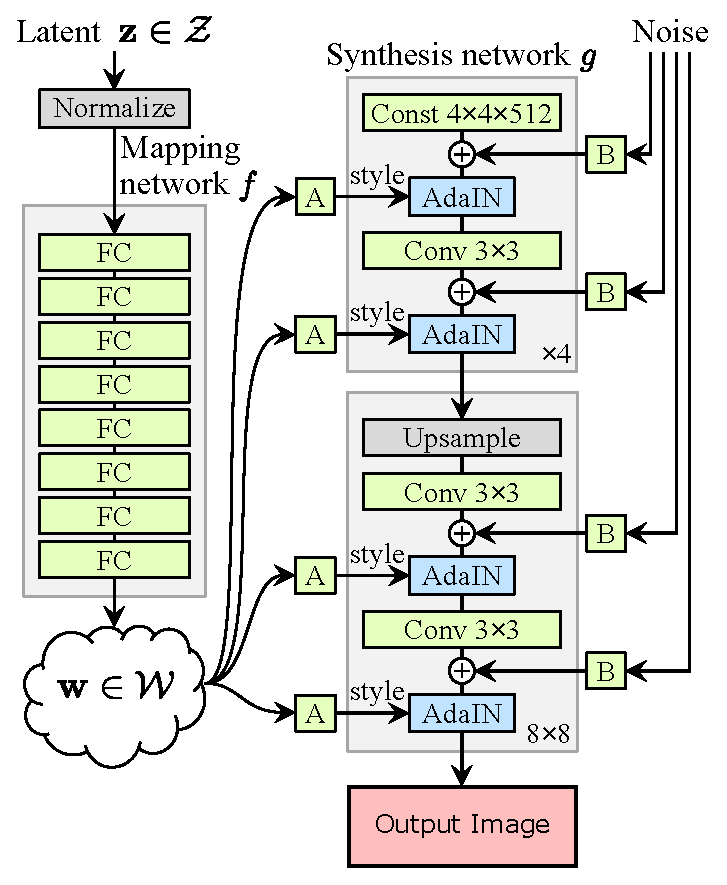
\includegraphics[width=0.75\linewidth]{figures/StyleGAN.eps}
  \caption{StyleGAN architecture for generation of a face image. Adapted from \cite{karras2019style}.}
  \label{fig:styleGAN}
\end{figure}

In case you cannot find the paper on arXiv, you can try to export the figure from the pdf or rebuild it. Taking a screenshot of the figure at the highest possible resolution works for presentations, but will lack quality in the printed version. 

\section{Tables}

Contents of a table can often be grouped. As illustrated by \autoref{tab:results}, vertical lines are not really necessary for that. Moreover, vertical lines often let the table seem overloaded. This is also described by the layout principle ''\textit{Less is more}''. Take a look at this \href{https://inf.ethz.ch/personal/markusp/teaching/guides/guide-tables.pdf}{Small Guide to Making Nice Tables}.
The best results for each metric should be made \textbf{bold}. Besides, note that the caption (in comparison to the figures) is above the table. 

If you work with Excel, \href{https://ctan.org/pkg/excel2latex}{this package} might be helpful for automatically generating \LaTeX -code. 

\begin{table}[H]
\caption{Results of metric 1, 2 and 3 in percent of our proposed methods in comparison with 3 baseline methods on benchmarks 1 and 2.}
\label{tab:results}  
\centering
\small
    \begin{tabular}{lLLLLRL}
    \toprule
          &      \multicolumn{2}{c}{Benchmark 1}     &      \multicolumn{4}{c}{Benchmark 2}     \\
          
\cmidrule(lr){2-3} \cmidrule(lr){4-7} 
          
    Method & \text{Metric 1} & \text{Metric 2} & \text{Metric 1} & \text{Metric 2} &  \multicolumn{2}{c}{Metric 3}  \\
    \midrule
    Baseline 1 \cite{baseline1} & 37.0    & \phantom{0}0.0     & 28.3  & \phantom{0}0.0     & \multicolumn{2}{C}{73.6}    \\
    Baseline 2 \cite{baseline2} & 84.1  & 36.9  & 81.3  & 29.9  & \multicolumn{2}{C}{93.1}  \\
    Baseline 3 & 85.2  & 60.1  & 83.6  & \textbf{57.2} & \multicolumn{2}{C}{-}   \\
        \midrule
    Ours 1 & 87.2  & 57.3  & 85.3  & 39.9  & 67.1 & \textbf{94.5} \\
    Ours 2 & \textbf{87.4} & \textbf{61.2} & \textbf{85.8} & 42.6  & 63.1 & 91.7  \\
    \bottomrule
    \end{tabular}%
\end{table}%

\section{Equations}
Number equations consecutively with equation numbers in parentheses. Make sure you follow the guidelines from \autoref{sec:notation}. Also, explain all used variables. When using vectors/matrices state the dimensions.

The scalar output $y$ of a single neuron with the activation function $\phi\left(\cdot\right)$ is defined as follows:
\begin{equation}
  y = \phi\left(\boldsymbol{w}^{\text{T}}\boldsymbol{x} + b\right)
  \label{eq:neuron}
\end{equation}
with the scalar $b$ denoting the bias, and $\boldsymbol{w}, \boldsymbol{x} \in \mathbb{R}^{512 \times 1}$ being the weight and the input of vectors of the neuron.

Note that there is no indentation as the sentences before and after the equation are connected. If you do not need to explain further variables, leave an extra line to start a new paragraph (with indentation).

\section{Captions}
Every figure needs to have a brief caption describing the figure/table. Do not write too much and keep it short. You should highlight the details and interpret them in the written text only. In contrast to the caption of a figure, the caption of the table is above the table. 


\section{Referencing}
All figures/tables need to be referenced in the written text. For convenience, use \verb'\autoref{fig:styleGAN}' to reference figures. This automatically adds the type of reference in front of the number:
\begin{itemize}
  \item \autoref{fig:styleGAN}
  \item \autoref{tab:results}
  \item \autoref{eq:neuron}
  \item \autoref{sec:notation}
  \item \autoref{ch:template_info}
\end{itemize}


\section{Clean Bibliography}

Every claim you make in the thesis must be verified by either your results or a citation. For details on how and what to cite please take look at \href{https://www.ub.tum.de/en/citation-guide}{TUM Citation Guide}. \textbf{If you fail to provide the source of a figure your thesis can be graded as fail 5,0 due to plagiarism.} Therefore, I recommend to always write down your source when you take a figure from another paper such that you will not forget citing it. You are on the safe side if you make all your figures by yourself. This also allows you to have an overall more consistent notation throughout the thesis. In the related work and background chapter, it is also fine to take figures from other papers (and improve them), but the source needs to be named! Examples are \autoref{fig:styleGAN} and \autoref{fig:faces}.

Go to \href{https://scholar.google.com/}{Google Scholar} and search for the paper you want to cite. You can copy the bibtex entry from there directly to your bibliography file so that all the references have the same look. 

Do not change the bibliography style. The first letter of the last name of the authors together with the last two digits of the year of publication should appear in the reference. Like this: \cite{baseline1} (= [EAO19])

Make sure the bibliography is consistent!
Never forget to mention author(s), title, year and where the article was published. Also, make sure every conference is formatted the same way and the title is written (capitalized) as in the paper (double \{\{Title you Want to Cite\}\} will do the job).

\section{\LaTeX\ Literature}
\label{sec:literature}
You will find many \LaTeX-tutorials searching the internet. Besides,   \cite{Ko03} is a quite comprehensive book, of which the library has adequate stock.